\subsection{MEC Architecture}

ETSI establishes a reference framework and architecture to realize MEC as shown below:

\begin{figure}[h!]
    \centering
    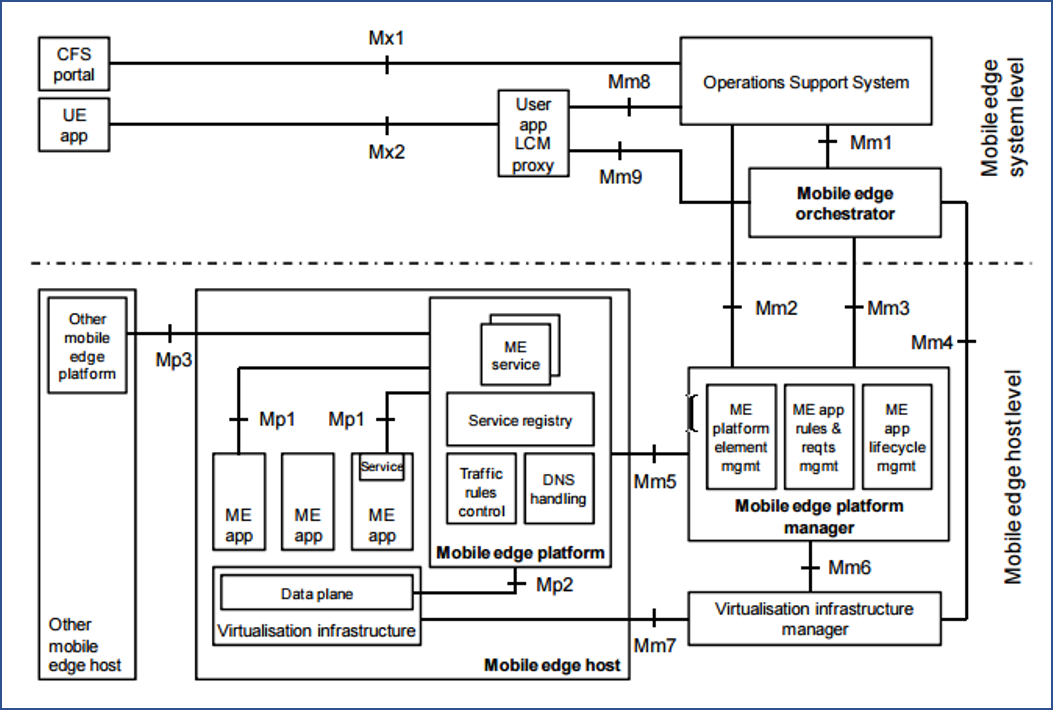
\includegraphics[width=0.9\textwidth]{mec_ref_architecture}
    \label{fig:figure4}
    \caption{ETSI MEC Reference Architecture}
\end{figure}

The architecture comprises the following 4 components:
\begin{enumerate}
    \item \textit{The MEC host} – provides the necessary infrastructure including virtualized resources.
    \item \textit{The MEC Platform} – Provides functionality and interfaces to run applications on top of the MEC host.
    \item \textit{MEC Management} – Handles host and system level management. It can be done at two levels – the host level involving the platform manager and the infrastructure manager and the system level using the MEC Edge orchestrator.
    \item \textit{MEC Applications} – Are services provided through the MEC architecture some of which can also be provided by the MEC platform manager.
\end{enumerate}
